\section{Private Capacity of Quantum Channels}

\begin{frame}{Private Capacity of a Wiretap Channel}
The private capacity $P(\mathcal{N})$ of a classical wiretap channel $\mathcal{N} = p_{Y,Z|X}$ is defined as follows.
\begin{tcolorbox}
$$P(\mathcal{N}) = \max_{p_{U,X}(u,x)} \left[ I(U;Y) - I(U;Z) \right]$$
\end{tcolorbox}

\begin{figure}
    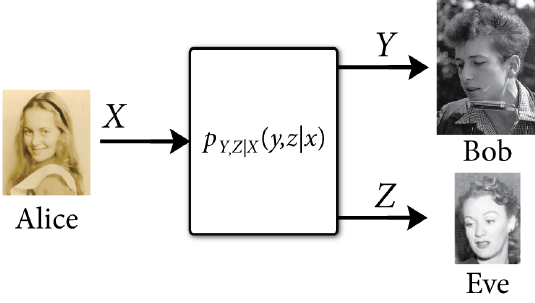
\includegraphics[width=0.4\textwidth]{figures/wiretap_channel.png}
    \caption{Classical wiretap channel.}
\end{figure}
\end{frame}

\begin{frame}{Properties: Private Capacity of a Wiretap Channel}
\begin{itemize}
    \setlength{\itemsep}{1.5em}
    \item Non-negativity
    $$P(\mathcal{N}) \geq 0$$
    \item Additivity
    $$P(\mathcal{N} \otimes \mathcal{M}) = P(\mathcal{N}) + P(\mathcal{M})$$
    \item Equivalence of asymptotic and single use capacity
    $$\lim_{n \rightarrow \infty} \frac{1}{n} P(\mathcal{N}^{\otimes n}) = P(\mathcal{N})$$
\end{itemize}
\end{frame}

\begin{frame}{Private Capacity of a Quantum Channel}
Consider a classical-quantum state of the form given below.
$$\rho_{XA'} = \sum_{x} p_X(x) \ket{x}\bra{x}_X \otimes \rho_{A'}^x $$

The private capacity $P(\mathcal{N})$ of a quantum channel $\mathcal{N}$ is defined as follows.
\begin{tcolorbox}
$$P(\mathcal{N}) = \max_{\rho_{XA'}} \left[ I(X;B)_\rho - I(X;E)_\rho \right]$$
\end{tcolorbox}
\end{frame}

\begin{frame}{Properties: Private Capacity of a Quantum Channel}
\begin{itemize}
    \setlength{\itemsep}{1.5em}
    \item Non-negativity
    $$P(\mathcal{N}) \geq 0$$
    \item Bounded by coherent information
    $$P(\mathcal{N}) \leq Q(\mathcal{N})$$
    \item Non-additivity
    $$P(\mathcal{N} \otimes \mathcal{M}) \neq P(\mathcal{N}) + P(\mathcal{M})$$
\end{itemize}
\end{frame}
